\section{The Analysis of Security and Privacy}
\label{sec:analysis}
In this section, we presents the analysis that UPPRESSO achieves the required properties of security and privacy.


\subsection{Security}
UPPRESSO satisfies with the four security requirements of identity tokens in SSO services,
     as listed in Section \ref{subsec:basicrequirements}.

%while the detailed process of proof is provided in the Appendix.
% ����汾���Ȳ��ܸ�¼��

\vspace{1mm}
\noindent\textbf{User Identification.}
The RP always derives an identical permanent account from different identity tokens binding $PID_U$ and $PID_{RP}$.
That is,
    in the user's any $i$-th and $i'$-th ($i \neq i'$) login instances to the RP,
 $\mathcal{F}_{Acct}(PID_{U}^i, PID_{RP}^i) = \mathcal{F}_{Acct}(PID_{U}^{i'}, PID_{RP}^{i'}) = [ID_U]ID_{RP}$


\vspace{1mm}
\noindent\textbf{RP Designation.}
An identity token binding $PID_U$ and $PID_{RP}$,
    designates the target RP, and only the target RP.
The RP calculates $PID_{RP}$ by itself with the trapdoor $t$ sent from the user,
    and checks $PID_{RP}$ in the identity token.
So the target RP will accept this token.
Meanwhile,
        the honest IdP guarantees, within its validity period, only one $PID_{RP}$ will be bound in some identity token.

\vspace{1mm}
\noindent\textbf{Confidentiality.}
There is no event leaking the identity tokens to any malicious entity other than the authenticated user and the designated RP.
First of all, the communications among the IdP, RPs and users,
    are protected by TLS,
    and the \verb+postMessage+ HTML5 API ensures the dedicated channels between two scripts within the user agent,
    so that adversaries cannot eavesdrop the transmission of identity tokens.
Meanwhile, the honest IdP sends the identity token only to the authenticated user,
    and this user forwards it to the RP through $Enpt_{RP}$.
The binding of $Enpt_{RP}$ and $ID_{RP}$ is ensured by the RP certificate,
so only the designated target RP receives this identity token.
%The detailed process of proof is shown in Appendix.

\vspace{1mm}
\noindent\textbf{Integrity.}
The identity token binds $ID_U$ and $ID_{RP}$,
    implicitly or explicitly, and any breaking will result in some failed check or verification.
The integrity is ensured by the IdP's signatures:
 (\emph{a}) the identity token binding $PID_U$ and $PID_{RP}$, is signed by the IdP,
  and (\emph{b}) the relationship between $PID_{RP}$ and $t$ (or collision-free $H(t)$) is also bound by the IdP's signature in the $PID_{RP}$ registration result.
Thus,
    $ID_U$ and $ID_{RP}$ are actually bound by the IdP's signatures,
        due to the one-to-one mapping between (\emph{a}) the pair of $ID_U$ and $ID_{RP}$ and (\emph{b}) the triad of $PID_U$, $PID_{RP}$, and $t$.

%The detailed process of proof is shown in Appendix.

%The detailed process of proof is shown in Appendix.



\subsection{Privacy}
We show that UPPRESSO effectively prevents the attacks of IdP-based login tracing and RP-based identity linkage.

\vspace{1mm}
\noindent\textbf{IdP-based Login Tracing.}
The information accessible to the IdP but derived from the RP's identity,
    is only $PID_{RP}$, where $PID_{RP} = [t]ID_{RP}$ is calculated by the user.
Because  (\emph{a}) $t$ is a number randomly chosen from $(1,n)$ by the user and kept secret to the IdP
 and (\emph{b}) $ID_{RP} = [r]G$ and $G$ is the base point,
 the IdP has to view $PID_{RP}$ as randomly chosen from $\mathbb{E}$.
So, the IdP cannot derive the RP's identity or link any pair of $PID_{RP}^i$ and $PID_{RP}^{i'}$,
    and the IdP-based identity linkage is impossible.

\vspace{1mm}
\noindent\textbf{RP-based Identity Linkage.}
We prove UPPRESSO prevents the RP-based identity linkage based on the elliptic curve decision Diffie-Hellman (ECDDH) assumption \cite{GoldwasserK16}.

++++

We briefly introduce the ECDDH assumption.
Let $\mathbb{E}$ be an elliptic curve over a finite field $\mathbb{F}_q$,
    and $P$ be a point on $\mathbb{E}$ of order $n$.
For any probabilistic polynomial time (PPT) algorithm $\mathcal{D}$,
 two probability distributions \{$[a]P$, $[b]P$, $[ab]P$\} and \{$[a]P$, $[b]P$, $[c]P$\}
are computationally indistinguishable,
 where $a$, $b$ and $c$ are integer numbers randomly and independently chosen from $(1,n)$.
That is,
    there is a negligible $\sigma(k)$ with the security parameter $k$ such that:


%Let $q$ be a large prime and $\mathbb{G}$ denotes a cyclic group of order $n$ of an elliptic curve $E(\mathbb{F}_q)$.
%Assume that $n$ is also a large prime. Let $P$ be a generator point of $\mathbb{G}$. 

%where $q$ and $n$ are large primitive number, and $P$ is the point of $\mathbb{G}$.
%For any probabilistic polynomial time (PPT) algorithm $D$, the distributions, \{$P$, $aP$, $bP$, $abP$\}$_{a,b \in \mathbb{Z}_n}$ and \{$P$, $aP$, $bP$, $cP$\}$_{a,b,c \in \mathbb{Z}_n}$, are computationally indistinguishable. There is a negligible $\sigma(k)$, where $k$ is the security parameter.
\begin{equation*}
Pr[\mathcal{D}(P, [a]P, [b]P, [ab]P)=1]-Pr[\mathcal{D}(P, [a]P, [b]P, [c]P)=1]=\sigma(k)
\end{equation*}

Let us see the data exposed to an RP.
The RP holds $ID_{RP}$,  generates $PID_{RP}$, $Acct$, and receives $t$, registration result (containing $PID_{RP}$, $H(t)$),
    and identity proof (including $PID_{RP}$ and $PID_U$).
The repetitive data should also be deleted, for example, $PID_{RP}$ is generated as $PID_{RP}= [t]{ID_{RP}}$ so that $PID_{RP}$ can be omitted (so as $Acct = [t^{-1}]PID_{U}$).
Finally, the effective date collected by the RP in each SSO login instance
 is $\langle ID_{RP}, t, PID_U\rangle$,
 while $PID_U = [ID_U][t]{ID_{RP}}$.

% ���̫���ˣ�����Ҫͼ
%\begin{figure*}
%  \centering
%  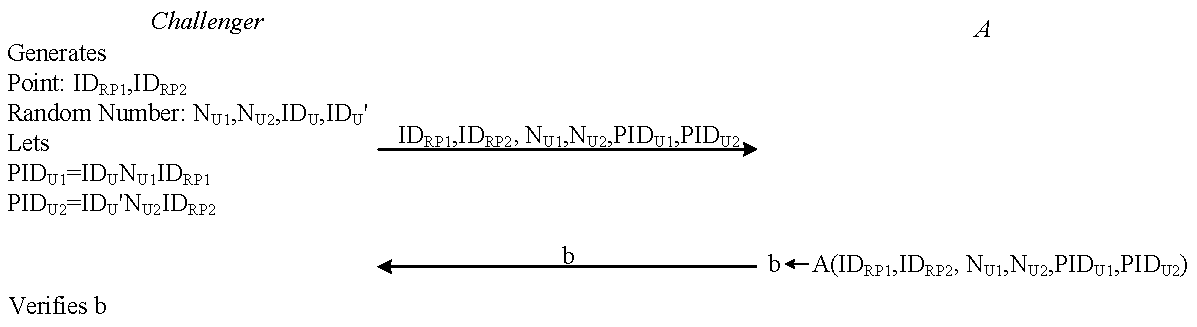
\includegraphics[width=0.82\linewidth]{fig/game1.pdf}
%  \caption{The Game.}
%  \label{fig:game}
%\end{figure*}


\begin{figure}[tb]
  \centering
  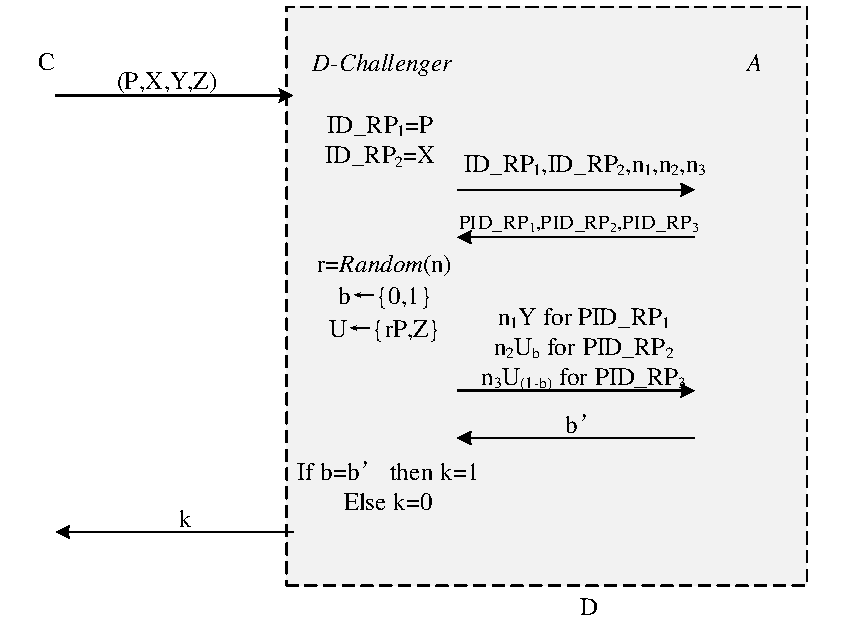
\includegraphics[width=1\linewidth]{fig/dalgorithm.pdf}
  \caption{The assumed algorithm based on the RP-based identity linkage.}
  \label{fig:dalgorithm}
\end{figure}

There is the data set, $\langle ID_{RP_j}$, $t_j$, $[ID_U][t_j]{ID_{RP_j}}\rangle$,
    $\langle ID_{RP_{j'}}$, $t_{j'}$, $[ID_{U'}] [t_{j'}] {ID_{RP_{j'}}}\rangle$, from two RPs ($RP_j$ and $RP_{j'}$),
that RP-based identity linkage attack can be considered as these collusive RPs guesses whether $ID_U$ equals $ID_{U'}$.

Here, we define the game $\mathcal{G}$, the adversary owns the same ability as collusive RPs.
The adversary receive the input $\langle ID_{RP_j}$, $t_j$, $[ID_U][t_j]{ID_{RP_j}}\rangle$,
    $\langle ID_{RP_{j'}}$, $t_{j'}$, $[ID_{U'}] [t_{j'}] {ID_{RP_{j'}}}\rangle$, from the challenger, and returns the result $s$.
The result is 1, when adversary guess that $ID_U = ID_{U'}$, otherwise $s=0$.
%The game is shown as Figure \ref{fig:game}.
The RP-based identity linkage attack is equivalent to
 adversary has the advantage on the guessing game (i.e., $Pr_1-Pr_2>\sigma(k)$).

We define $Pr_s$ is the probability, while the adversary returns $s=1$ as $ID_U$ equals to $ID_{U'}$ (i.e., the attack succeeds).
 And $Pr_{\bar{s}}$ is the probability, while the adversary returns $s=1$ but $ID_U$ does not equal to $ID_{U'}$ (i.e., the attack fails).
Adversary has the advantage on the game means that
\begin{equation*}
Pr_s-Pr_f>\sigma(k)
\end{equation*}

We design a PPT algorithm $\mathcal{D}^*$ based on $\mathcal{G}$, shown in Figure \ref{fig:dalgorithm}.
The input of $\mathcal{D}^*$ in the form $(Q_1, Q_2, Q_3, Q_4)$, while $Q_i$ are points on $\mathbb{E}$.
The challenger receives the input,
    randomly chooses $t_j$ and $t_{j'}$ from $(1,n)$,
    and set $ID_{RP_j}=Q_1$, $ID_{RP_{j'}}=Q_2$, $PID_{U,j}=[t_j]Q_3$, and $PID_{U',j'}= [t_{j'}] Q_4$.
The challenger input $<Q_1, t_j, [t_j]Q_3>$ $<Q_2, t_{j'}, [t_{j'}] Q_4>$ to the game $\mathcal{G}$.
At the end, $\mathcal{D}^*$ returns the $s$ from the adversary as the result.

We let ($P$, $[a]P$, $[b]P$, $[ab]P$) and  ($P$, $[a]P$, $[b]P$, $[c]P$) be two inputs.
Thus there is
\begin{multline*}
\ \ \ \ \ \ \ \ \ \ \ \ \ \ \ \ \ Pr[\mathcal{D}^*(P,[a]P,[b]P,[ab]P)=1]=\\ Pr[\mathcal{G}(P, t_j, [t_j][b]P, aP, t_{j'},[t_{j'}][ab]P)=1]=Pr_s\\
\\
Pr[\mathcal{D}^*(P,aP,bP,cP)=1]=\ \ \ \ \ \ \ \ \ \
\\ Pr[\mathcal{G}(P, t_j, [t_j][b]P, aP, t_{j'},[t_{j'}][c/a] [a]P)=1]=Pr_f
\end{multline*}
in the first equation $ID_{U} = ID_{U'} = b$, so it is $Pr_s$
 while in the second equation $ID_{U} =b$ but $ID_{U'} = c/a$ so it is $Pr_f$.


Adversary has the advantage on the game means $Pr_1-Pr_2>\sigma(k)$,
    which violate the ECDDH assumption.
So an adversary cannot have the advantage on the game,
    and the RP-based identity linkage is computationally impossible.

